\section{Utility}


\subsection{Consumer Preferences}

\slide{Utility and Preferences}{
    Preferences allow us to rank bundles by choosing between two bundles. Now, however,
    we want to move towards finding the bundle that gives us the most satisfaction or pleasure.

    To do this, we introduce utility. In essence, utility is the satisfaction derived
    from consuming a good or service.

    We can construct a utility function to compare bundles:
    \begin{itemize}
        \item A utility function assigns a number to every possible consumption bundle.
        More preferred bundles are assigned a higher number than less preferred bundles.
        \item \((x_1, x_2) \succeq (y_1, y_2)\) if and only if \(u(x_1, x_2) \geq u(y_1, y_2)\).
    \end{itemize}
}

\slide{Ordinal and Cardinal Utility}{
    In these slides, the utility is an ordinal concept, not a cardinal concept.
    Meaning that the order matters, not the magnitude.

    Theories of utility that attach a significance to the magnitude of utility
    are known as \textbf{cardinal utility}. The size of the utility difference between two bundles of
    goods is supposed to have some sort of significance.

    On the other hand, when we order two bundles based on which is chosen,
    we assign an \textbf{ordinal utility} to the two bundles of goods: we just assign a higher 
    utility to the chosen bundle than to the rejected bundle. Any assignment that
    does this will be a utility function.

    We will stick with a purely ordinal utility framework.
}


\slide{Ordinal Utility}{
    If bundle X is weakly preferred to Y, then any valid utility function must assign a number
    at least as high to X as to Y.

    For example, \(U(\text{1 unit of coffee}) = 10\), \(U(\text{1 unit of cookies}) = 0\), and
    \(U(\text{1 unit of oatmeal}) = -5\) represents the same preferences as \(X \succeq Y\), 
    \(Y \succeq Z\), and \(X \succeq Z\).

    We only care about the rank of utilities; the actual numbers are less important. Furthermore,
    a utility function that preserves the rank will preserve the underlying preferences:
    \[U(coffee) = 1000, U(cookies) = 999, U(oatmeal) = 998\]
    is just as good as
    \[U(coffee) = 10, U(cookies) = 0, U(oatmeal) = -5.\]
}


\subsection{Monotonic Transformations}

\slide{Monotonic Transformations}{
    An increasing monotonic transformation is a function \(g(x)\) such that \(g(a) \geq g(b) \iff a \geq b\).

    Any strictly increasing monotonic transformation of a utility function represents the same preferences as
    the original utility function.

    This is because an increasing function will preserve the rank of the utilities, and therefore preserve
    the same preferences.

    If \(X \succ Y\) and \(g(X) > g(Y)\), where \(g\) is a monotone increasing function, then
    \(g(u(x_1, x_2))\) is an equivalent utility function to \(u(x_1, x_2)\).
}


\slide{Example}{
    Consider the ``doubling function'' which is a positive monotonic transformation: \(v(\cdot) = 2u(\cdot)\).
    This preserves the ranking of the bundles.

    If \(u(x_1, x_2) = 10\) and \(u(y_1, y_2) = 2\), then \(g(u(x_1, x_2)) = 20\) and \(g(u(x_1, x_2)) = 4\).
    Needless to say, \(g(u(x_1, x_2)) > g(u(y_1, y_2))\).
    
    Therefore, \(X \succ Y\), and the ordering (or ranking) is preserved.

    Other examples include: \(\ln(x)\), \(e^x\), \(cx\) where \(c > 0\), etc. In essence, any function whose
    first derivative is positive, can be considered a monotonic transformation.
}


\subsection{Indifference Curves and Utility}

\slide{Indifference Curves and Utility}{
    Consider a utility function \(u(x_1, x_2) = x_1 x_2\).
    \begin{itemize}
        \item Fix a level of utility \(k\) and find all combinations of \(x_1\) and \(x_2\) that give that level of utility.
        \item Changing the level \(k\) produces different indifference curves.
        \item To draw the indifference curves, we draw \emph{level sets} of the utility function, that is, the set of all
        \((x_1, x_2)\) such that \(u(x_1, x_2)\) is constant.
    \end{itemize}
    \[u(x_1, x_2) = k = x_1 x_2\]
    \[x_2 = \frac{k}{x_1}\]
}


\subsection{Different Utility Functions}

\slide{Utility of Perfect Substitutes}{
    If two goods are perfect substitutes, then it does not matter which good I buy as they will provide
    me with the same utility.

    All that matters to me is the total quantity I have: \(u(x_1, x_2) = x_1 + x_2\).

    More generally, they will provide the same rate of utility:
    \[u(x_1, x_2) = ax_1 + bx_2\]
    Here, \(a\) and \(b\) measure the value of goods \(x_1\) and \(x_2\) to the consumer.

    The slope of a typical indifference curve is: \(\frac{-a}{b}\).
}


\slide{Utility of Perfect Complements}{
    If two goods are perfect complements, then I consume them in a certain proportion.

    The general form of the indifference curves is:
    \[u(x_1, x_2) = \min \{ax_1, bx_2\}\]

    Here, \(a\) and \(b\) are positive and represent the proportion in which the goods
    are consumed. For example, \(a=1\) and \(b=1\) for right and left shoes.
}


\slide{Quasi-Linear Utility Functions}{
    Quasilinear utility functions have two a linear component and a non-linear component.
    The general form is:
    \[u(x_1, x_2) = v(x_1) + x_2\]
    Here, \(v(x_1)\) is the non-linear component. This function is linear in good 2 and
    non-linear in good 1.
}


\slide{Quasi-Linear Utility Functions}{
\begin{center}
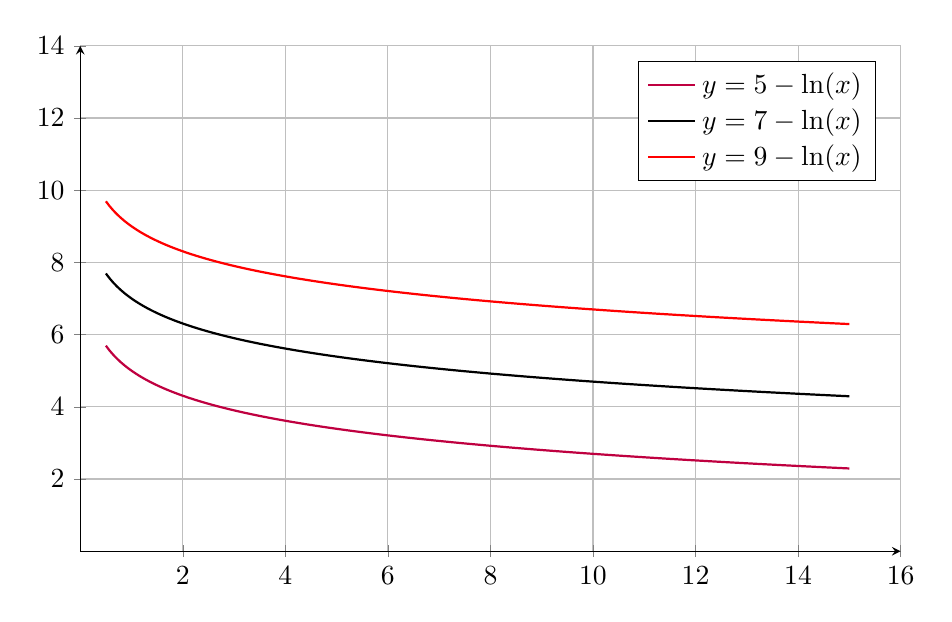
\begin{tikzpicture}
\begin{axis}[
    domain=0.5:15,
    samples=200,
    grid=both,
    width=12cm,
    height=8cm,
    xmin=0, xmax=16,
    ymin=0, ymax=14,
    axis lines=middle,
    xlabel={},
    ylabel={},
    legend style={at={(0.97,0.97)},anchor=north east}
]
\addplot[thick, purple] {5 - ln(x)};
\addlegendentry{$y = 5 - \ln(x)$}

\addplot[thick, black] {7 - ln(x)};
\addlegendentry{$y = 7 - \ln(x)$}

\addplot[thick, red] {9 - ln(x)};
\addlegendentry{$y = 9 - \ln(x)$}
\end{axis}
\end{tikzpicture}
\end{center}
}


\slide{Cobb-Douglas Utility Functions}{
    Cobb-Douglas utility functions embody the `well-behaved' preferences assumption.
    They have the general form:
    \[u(x_1, x_2) = x_1^{\alpha} x_2^{\beta}\]

    This is, arguably, the most important form of the utility function.
    
    Its slope is the marginal rate of substitution (MRS) for a consumer with `well-behaved'
    preferences.
}


\slide{Cobb-Douglas Utility Functions}{
\begin{center}
    \includegraphics[scale=0.475]{CB1}
\end{center}
}

\slide{Cobb-Douglas Utility Functions}{
    To get the slope of the function, we must differentiate:
    \[u(x_1, x_2) = x_1^{\alpha} x_2^{\beta}\]

    This is unnecessarily tedious. It is much easier to differentiate it after applying
    a monotonic transformation like the natural logarithm.

    Let's call the new function \(v(x_1, x_2) = g(u(x_1, x_2))\), where \(g\) is a monotonic transformation,
    i.e. the natural logarithm.

    \[v(x_1, x_2) = \ln(x_1^{\alpha} x_2^{\beta}) = \ln(x_1^{\alpha}) + \ln(x_2^{\beta})
    = \alpha \ln(x_1) + \beta \ln(x_2)\]

    Now, we can find the rate of change in utility with respect to \(x_1\) and \(x_2\).
    The next topic (MRS) will discuss precisely this.
}